\documentclass[10pt,letterpaper,subeqn]{beamer}
\setbeamertemplate{navigation symbols}{}
\usefonttheme{serif}
\usecolortheme{seahorse}


\usepackage{amsmath}
\usepackage{amsfonts}
\usepackage{amssymb}
\usepackage[english]{babel}
\selectlanguage{english}
\usepackage{bm}
\usepackage{booktabs}
\usepackage{color}
\usepackage[update,prepend]{epstopdf}
\usepackage{eqnarray}
\usepackage{framed}
\usepackage{fleqn}
\usepackage{graphics}
\usepackage{hyperref}
\usepackage[utf8]{inputenc}
\usepackage{setspace}
\usepackage{textcomp}
\usepackage{tcolorbox}
\usepackage{wrapfig}
\usepackage{multirow}
\usepackage{caption}
\usepackage{subcaption}
\usepackage{subfloat}
\setbeamertemplate{caption}[numbered]
\usepackage{wrapfig}
\usepackage{tikz}

\definecolor{cadmiumgreen}{rgb}{0.0, 0.42, 0.24}


%================================================================================
%== TITLE, NAMES, DATE
%================================================================================
\title{Estimating Difference-in-Differences in the Presence of Spillovers}
%\subtitle{Theory and Application to Contraceptive Reforms in Latin America}
\author{Damian Clarke\inst{\dag} }
\institute{\inst{\dag}  University of Oxford}
\date{August 2015}


%================================================================================
%== Document
%================================================================================
\begin{document}


\begin{frame}
\titlepage
\end{frame}
%================================================================================

\section{Introduction}
\begin{frame}[label=int1]
  \frametitle{This Paper}

\end{frame}

\section{Introduction}
\begin{frame}[label=int2]
  \frametitle{This Paper}

\end{frame}



%================================================================================
\section{Motivation}
\begin{frame}[label=motivation]
  \frametitle{Motivation}

\end{frame}

\begin{frame}[label=DDM]
  \frametitle{Difference-in-differences in Economics}
\begin{itemize}
 \item 
 \item 
 \item Consistency relies on the Stable Unit Treated Value Assumption (SUTVA)
 \item Much recent discussion within and outside of academics (eg ``The Worm Wars'')
\end{itemize}
\end{frame}

\begin{frame}[label=teenPreg]
  \frametitle{Teenage Pregnancy in Latin America}

\end{frame}



%================================================================================
\section{Methodology}
\begin{frame}[label=method1]
  \frametitle{Methodology}
``Typical'' diff-in-diff where outcome is generated by components of variance 
process (Ashenfelter and Card, 1985):
\vspace{4mm}
\begin{equation}
\label{Seqn:COV}
Y(i,t)=\delta(t) + \alpha D(i,t)+\eta(i)+\nu(i,t),
\end{equation}
\vspace{4mm}
and estimand of interest is:
\vspace{4mm}
\begin{eqnarray}
\label{Seqn:DD}
\alpha&=\{E[Y(i,1)|D(i,1)=1]-E[Y(i,1)|D(i,1)=0]\} \\ \nonumber
      &-\{E[Y(i,0)|D(i,1)=1]-E[Y(i,0)|D(i,1)=0]\}
\end{eqnarray}
\end{frame}

\begin{frame}[label=method2]
  \frametitle{Methodology}
This relies on a binary measure of treated versus non-treated.  In this paper,
I generalise this.  Consider:
\vspace{5mm}
\begin{equation}
\label{Seqn:COV2}
Y(i,t)=\delta(t) + \alpha D(i,t)+\textcolor{red}{\beta R(i,t)}+\eta(i)+\nu(i,t)
\end{equation}
\vspace{3mm}
where
\vspace{3mm}
\[
 R(i,t) =
  \begin{cases}
   f\Big(X(i,t)\Big)>0   & \text{if close to, but not in, treatment area} \\ 
   0                            & \text{otherwise} 
  \end{cases}
\]

\end{frame}

\begin{frame}[label=method3]
  \frametitle{Methodology}
\begin{itemize}
\item Here $X(i,t)$ is an observed measure of `distance'
\item And $f(\cdot)$ is a positive monotone function
\item However, $R(i,t)$ is not observed given that ``close'' is subjective
\end{itemize}
\end{frame}


\begin{frame}[label=method4]
  \frametitle{Methodology}
And this leads to two estimands:
\begin{eqnarray}
\nonumber
\label{Seqn:DDa}
\alpha&=\{E[Y(1)|D(1)=1,R(1)=0]-E[Y(1)|D(1)=0,R(1)=0]\} \\ \nonumber
      &\ -\ \{E[Y(0)|D(1)=1,R(1)=0]-E[Y(0)|D(1)=0,R(1)=0]\}, 
\end{eqnarray}

\begin{eqnarray}
\nonumber
\beta&=\{E[Y(1)|D(1)=0,R(1)\neq 0]-E[Y(1)|D(1)=0,R(1)=0]\} \\ \nonumber
      &\ -\ \{E[Y(0)|D(1)=0,R(1)\neq 0]-E[Y(0)|D(1)=0,R(1)=0]\}. 
\end{eqnarray}
\vspace{3mm} \\
where $i$ has been supressed for ease of exposition.
\end{frame}

%================================================================================
\section{Estimation}
\begin{frame}[label=estim1]
  \frametitle{Estimation}
In this paper I am interested in estimating the unbiased causal effects $\alpha$ 
and $\beta$.  This is referred to as a ``spillover robust double differences
estimator''
\vspace{4mm}
\begin{itemize}
\item This allows for spillovers, without imposing that they must exist
\item More importantly, if spillovers do exist, this corrects for potential 
confounding effects of including ``close'' units in the control group
%\item 
\end{itemize}
\end{frame}

\begin{frame}[label=estim2]
  \frametitle{Estimation}
In a Rubin (1974) causal framework, $Y^1(i,t)$ is the potential outcome for some 
person $i$ at time $t$ if they were to receive treatment, and $Y^0(i,t)$ if the 
person were not to receive treatment.
\vspace{4mm}
\begin{itemize}
\item The fundamental challenge of inference is that only one of these is observed
\item Inference then proceeds using expectations over groups
\item Unbiasedness relies on parallel trend assumptions holding
\end{itemize}
\end{frame}

\begin{frame}[label=estim3]
  \frametitle{Estimation}
Hence, I define:
\vspace{4mm}
\begin{eqnarray}
\label{Seqn:estimATT}
ATT=E[Y^1(i,1)-Y^0(i,1)|D(i,1)=1]\  \\
\label{Seqn:estimATC}
ATC=E[Y^1(i,1)-Y^0(i,1)|C(i,1)=1],
\end{eqnarray}
\vspace{4mm} \\
where $C(i,t)$ refers to close, and is simply a re-definition of $R(i,t)$:
$C(i,t)=\mathbf{1}_{R(i,t)\neq 0}$
\vspace{4mm} \\
\begin{enumerate}
\item[ATT] Average treatment effect on the treated
\item[ATC] Average treatment effect on the close to treated
\end{enumerate}
These are the sample counterparts of $\alpha$ and $\beta$, the population 
estimands of interest.

\end{frame}



\begin{frame}[label=estim4]
  \frametitle{Estimation}
\textbf{Unbiasedness} relies on a number of assumptions. \\
\vspace{5mm}

\begin{tcolorbox}[title =1. Parallel trends in treatment and control]
$E[Y^0(1)-Y^0(0)|D(1)=1,C(1)=0]= \\
E[Y^0(1)-Y^0(0)|D(1)=0,C(1)=0]$
\end{tcolorbox}

\begin{tcolorbox}[title =2. Parallel trends in close and control]
$E[Y^0(1)-Y^0(0)|D(1)=0,C(1)=1]= \\
E[Y^0(1)-Y^0(0)|D(1)=0,C(1)=0]$
\end{tcolorbox}

\end{frame}


\begin{frame}[label=estim5]
  \frametitle{Estimation}
This is the fundamental diff-in-diff identifying assumption of parallel trends, 
generalised to hold for treatment \emph{and} close to treatment status
\vspace{4mm} \\
\begin{itemize}
\item However, note that we no longer need to make \emph{any} assumptions 
regarding parallel trends between treatment and close to treatment units
\item This allows for direct interactions of any form between those living in 
treatment areas, and those living close by
\item This loosens SUTVA, however, as a matter of course, some reduced form of 
SUTVA must be assumed for causal estimates
\end{itemize}
\end{frame}


\begin{frame}[label=estim6]
  \frametitle{Estimation}
\begin{tcolorbox}[title =3. SUTVA holds for some units]
There is some subset of individuals $j\in J$ of the total population $i\in N$ 
for whom potential outcomes ($Y_j^0, Y_j^1$) are independent of the treatment 
status $D=\{0,1\}\ \forall_{i\neq j} \in N$.
\end{tcolorbox}
\vspace{4mm}
This loosens SUTVA in the sense that here it must hold only between \emph{some}
units.  Identification relies on there existing at least some subset of units 
which are not affected by the treatment status of others.
\end{frame}


\begin{frame}[label=estim7]
  \frametitle{Estimation}
Finally, it is assumed that spillovers, or violations of SUTVA, do not occur 
randomly in the population
\vspace{4mm}
\begin{tcolorbox}[title =4. Assignment to close to treatment depends on observable $X$]
There exists an assignment rule $\delta\Big(X(i,t)\Big)=\{0,1\}$ which maps 
individuals to close to treatment status $C(i,t)$, where $\delta\Big(X(i,t)\Big)=
\mathbf{1}_{X(i,t)<d}$, $X(i,t)$ is an observed covariate, and $d$ is a fixed
scalar cutoff. 
\end{tcolorbox}
\end{frame}


\begin{frame}[label=estim8]
  \frametitle{Estimation}
This is quite demanding.  It requires that spillovers be based on an observable 
and unidimensional factor (though of arbitrary functional form)
\vspace{4mm}
\begin{itemize}
\item In some cases this may be acceptable (ie physical distance)
\item In other cases, we will be interested in extending this to allow for 
multidimensional determinants, or interactions between distance and individual
characteristics
\item A multidimensional (non-parametric) extension of this methodology is 
provided in the paper
\end{itemize}
\end{frame}

\begin{frame}[label=estim8]
  \frametitle{Estimation}
\begin{tcolorbox}[title =Proposition 1]
Under assumptions 1 to 4, the ATT and ATC can be 
consistently estimated by least squares when controlling, parametrically or
non-parametrically, for $C(i,t)=\mathbf{1}_{X(i,t)\leq d}$.
\end{tcolorbox}
\end{frame}

%================================================================================
\section{Empirical Application}
\begin{frame}[label=empir1]
  \frametitle{Empirical Application}
In order to examine this empirically, we need:
\vspace{4mm}
\begin{enumerate}
\item A sharply defined policy reform over space and time
\item A treatment group and control group seperated by geographic boundaries
\item Members of the treatment group with sufficient incentives to violate their
status, travelling to (or otherwise managing to access) the reform
\end{enumerate}
\end{frame}

\begin{frame}[label=empir2]
  \frametitle{Empirical Application}
As such, we focus on two recent contraceptive reforms:
\vspace{6mm}
\begin{enumerate}
\item \textbf{Chile} 2008 reform: The emergency contraceptive pill
\item \textbf{Mexico} April 26, 2007: Legal interruption of pregnancy (ILE)
\end{enumerate}
\vspace{6mm}
These reforms work well: the costs of not having access (undesired pregnancy) are
very high, and geographic boundaries (comunas, municipios) can be crossed easily
\end{frame}


\subsection{Empirical Application 1: Emergency Contraception in Chile}
\begin{frame}[label=empirA]
  \frametitle{Empirical Application 1: Emergency Contraceptive Pill in Chile} 
In 2008, following years of constitutional challenges, the decision of whether
or not to prescribe the morning after pill was left in the hand of the mayor of
each comuna in Chile
\vspace{5mm}
\begin{itemize}
\item This was codified in the \emph{Normas Nacionales sobre Regulaci\'on de la 
Fertilidad}
\item I collect data on all births (DEIS), population (INE) and whether the 
morning after pill was prescribed by comuna (Dides et al.)
\item Further details and \hyperlink{ChileDesc}{\textcolor{blue}{descriptives}} provided 
in Bentancor and Clarke (2014) and Casas Becerra (2008)
\end{itemize}
\end{frame}

\begin{frame}[label=empirA1]
%  \frametitle{Emergency Contraceptive Pill in Chile} 
\begin{figure}
\begin{center}
\caption{Trends in Teenage Pregnancy (Chile)}
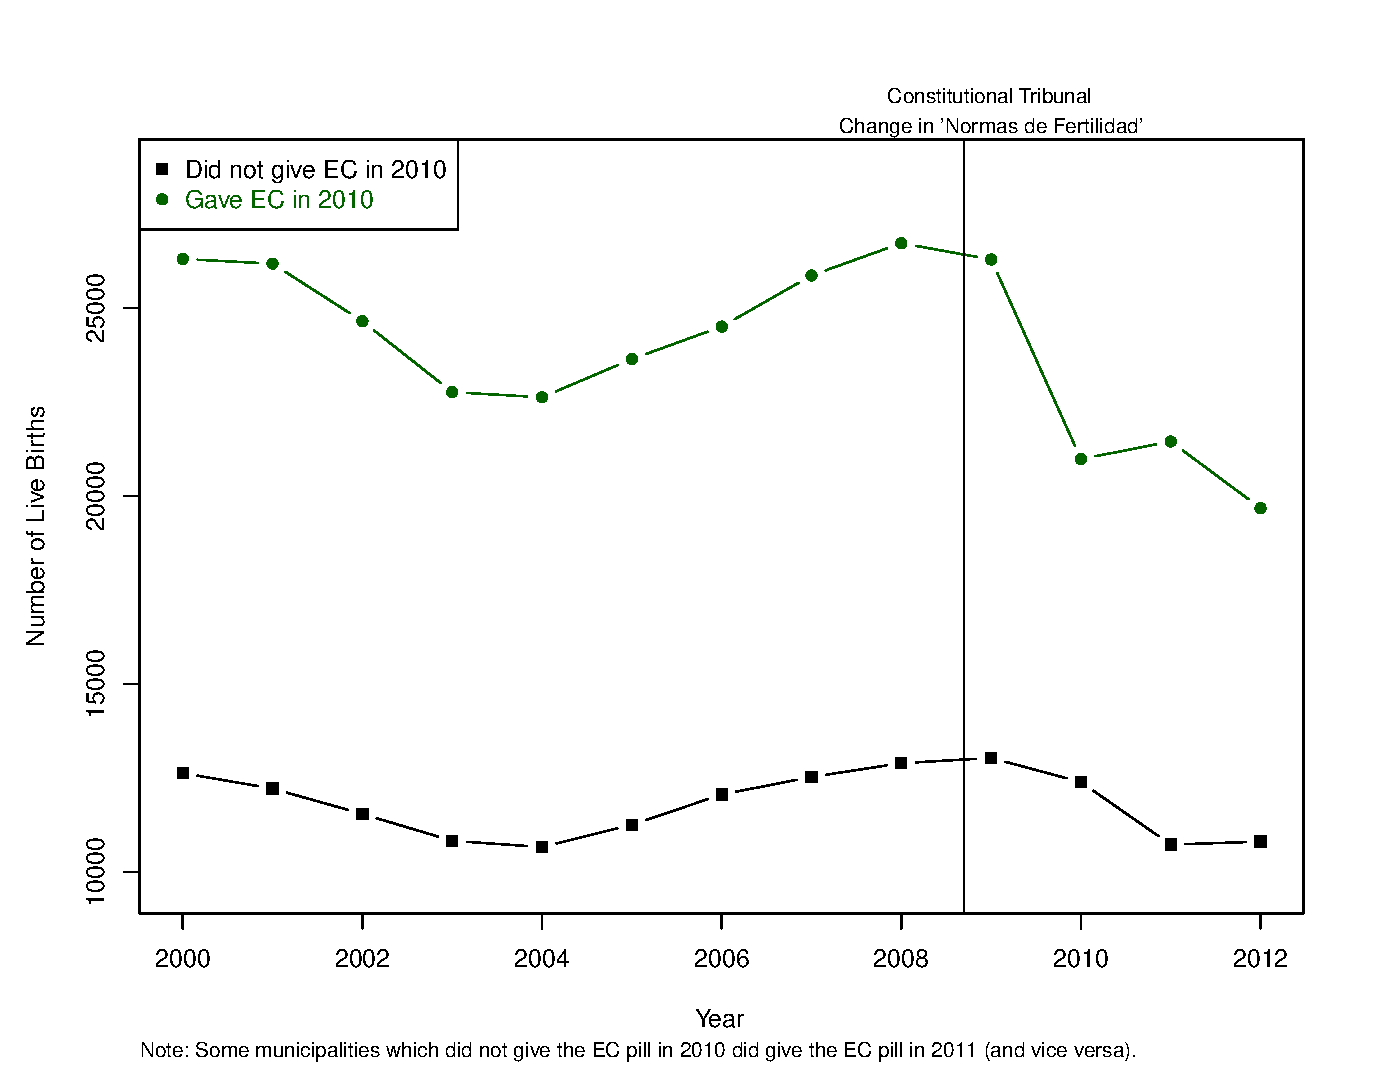
\includegraphics[scale=0.45]{./figures/Reform1519.eps}
\end{center}
\end{figure}
\end{frame}

\begin{frame}[label=empirA2]
%  \frametitle{Emergency Contraceptive Pill in Chile}
\begin{table}[htpb!]
\caption{Treatment Effects and Spillovers: Chile (15-19 year olds)}
\vspace{-2mm}
\label{Stab:spill1519}
\begin{center}
\scalebox{0.8}{
\begin{tabular}{lccccc} \toprule
&Pr(Birth)&Pr(Birth)&Pr(Birth)&Pr(Birth)&Pr(Birth)\\
&(1)&(2)&(3)&(4)&(5)\\ \midrule
&&&&& \\
Treatment&$-$0.046$^{***}$&$-$0.058$^{***}$&$-$0.066$^{***}$&$-$0.073$^{***}$&$-$0.074$^{***}$\\
&(0.011)&(0.013)&(0.014)&(0.014)&(0.015)\\
Close 1&&$-$0.049$^{***}$&$-$0.056$^{***}$&$-$0.062$^{***}$&$-$0.062$^{***}$\\
&&(0.015)&(0.014)&(0.014)&(0.014)\\
Close 2&&&$-$0.040$^{*}$&$-$0.047$^{*}$&$-$0.048$^{**}$\\
&&&(0.023)&(0.024)&(0.024)\\
Close 3&&&&$-$0.038$^{*}$&$-$0.038$^{*}$\\
&&&&(0.023)&(0.023)\\
Close 4&&&&&$-$0.014\\
&&&&&(0.023)\\
& & & & & \\
Mean&0.052&0.052&0.052&0.052&0.052\\
Regions$\times$ Time&1,929&1,929&1,929&1,929&1,929\\ \midrule
\multicolumn{6}{p{12.4cm}}{\begin{footnotesize}\textsc{Notes}:     
Each column represents a separate difference-in-differences regression
 including full time and municipal fixed effects and linear trends by 
municipality. Standard errors are clustered at the level of the       
geographic region of treatment (municipality). Close variables are    
included in bins of 10km, so Close 1 refers to distances of [0,10)km, 
Close 2 refers to [10,20)km, and so forth. Models are estimated using 
a binary (logit) model for birth versus no birth. Coefficients are    
expressed as log odds.\end{footnotesize}}\\
\bottomrule\end{tabular}}\end{center}\end{table}

\end{frame}

\begin{frame}[label=empirA3]
  \frametitle{Emergency Contraceptive Pill in Chile}
The effect sizes are quite large.  There are a few things to consider:
\vspace{4mm}
\begin{itemize}
\item Roe vs Wade in USA:
\begin{itemize}
\item Bailey (2006) \hspace{4.4cm}-0.093 (0.043)
\item Guldi (2008)  \hspace{4.4cm} -0.100 (0.054)
\item Ananat and Hungerman (2012) \hspace{1.75cm} -0.043 (0.015)
\end{itemize}
\item Contraceptive Pill in USA:
\begin{itemize}
\item Bailey (2006) \hspace{4.4cm}-0.074 (0.057)
\item Guldi (2008)  \hspace{4.4cm} -0.085 (0.041)
\item Ananat and Hungerman (2012) \hspace{1.75cm} -0.088 (0.022)
\end{itemize}
\item Morning after pill in USA: 
\begin{itemize}
\item \hyperlink{GrossEtAl}{\textcolor{blue}{Gross et al (2014)}} \hspace{3.7cm} -0.020 (0.020)
\end{itemize}
\item 16 and Pregnant in USA: 
\begin{itemize}
\item Kearney and Levine (2014) \hspace{2.8cm} -0.057
\end{itemize}
\end{itemize}

\end{frame}

\begin{frame}[label=empirA4]
%  \frametitle{Emergency Contraceptive Pill in Chile}
\begin{figure}
\begin{center}
\caption{Placebo Test 1: Parallel Trends Between Treatment and Control}
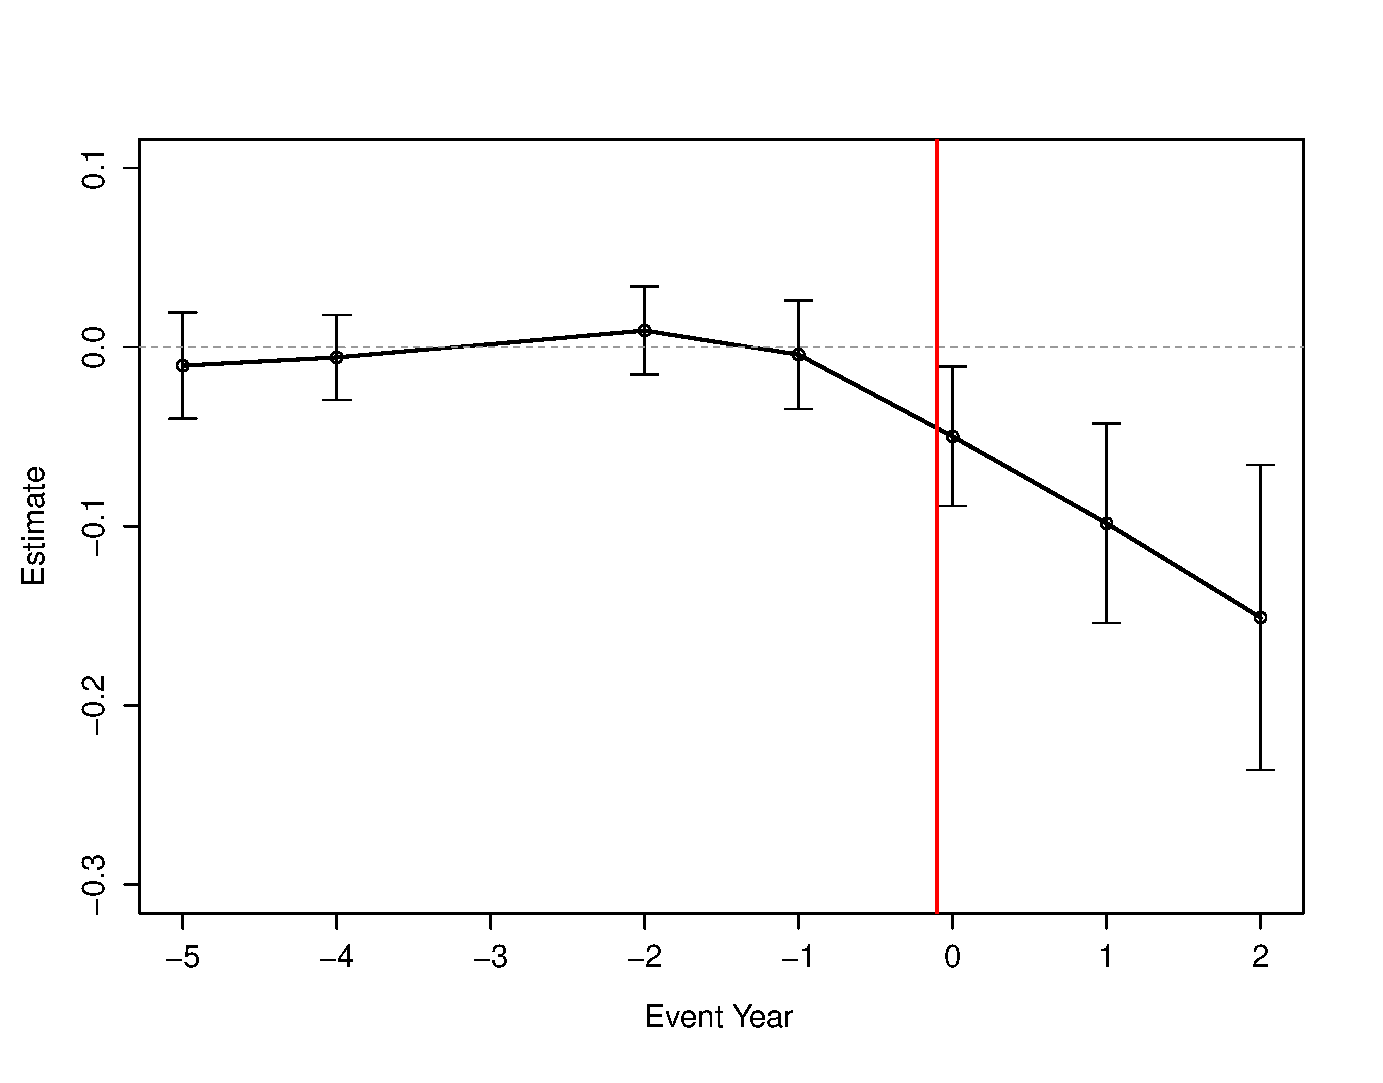
\includegraphics[scale=0.45]{./figures/Event1519treat.eps}
\end{center}
\end{figure}
\end{frame}

\begin{frame}[label=empirA5]
%  \frametitle{Emergency Contraceptive Pill in Chile}
\begin{figure}
\begin{center}
\caption{Placebo Test 1: Parallel Trends Between Close and Control}
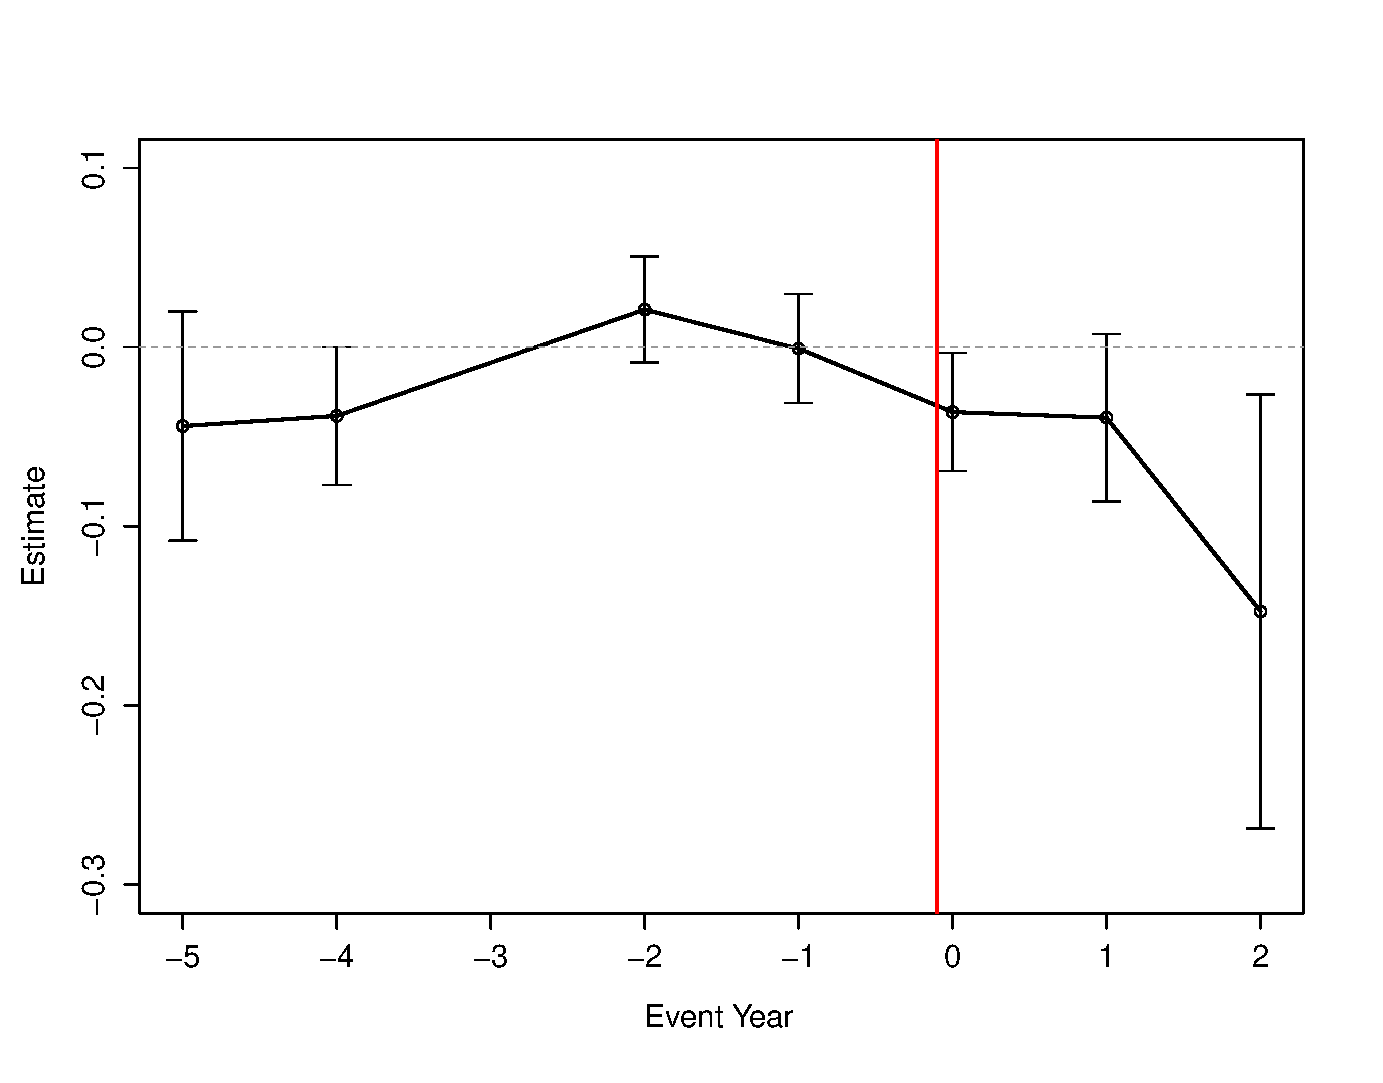
\includegraphics[scale=0.45]{./figures/Event1519close.eps}
\end{center}
\end{figure}
\end{frame}




\subsection{Empirical Application 2: Legal Interuption of Pregnancy in Mexico DF}
\begin{frame}[label=empirB]
  \frametitle{Empirical Application 2: Legal Interuption of Pregnancy in Mexico DF}
On April 26, 2007 the legislative assembly of Mexico DF voted to legalise legal 
interruption of pregnancy (ILE) whenever requested by the woman up to 12 weeks of 
gestation, reforming article 144 of the penal code of Mexico DF
\vspace{5mm}
\begin{itemize}
\item This made Mexico DF one of the most liberal areas in terms of abortion
contraception in all of Latin America (Fraser, Lancet 2015)
\item I collect data on births (INEGI), and municipio controls
\item Further \hyperlink{MexicoDesc}{\textcolor{blue}{descriptive statistics}}.
\end{itemize}

\end{frame}

\begin{frame}[label=empirB2]
%  \frametitle{Emergency Contraceptive Pill in Mexico}
\begin{table}[h!]
\begin{center}
\caption{Treatment Effects and Spillovers: Mexico (15-19 year olds)}
\label{Stab:Mex1519}
\scalebox{0.7}{
\begin{tabular}{lccccc} \toprule
 & N Birth & N Birth & N Birth & N Birth & N Birth  \\ 
 & (1) & (2) & (3) & (4) & (5)  \\ \midrule
\vspace{4pt} & \begin{footnotesize}\end{footnotesize} & \begin{footnotesize}\end{footnotesize} & \begin{footnotesize}\end{footnotesize} & \begin{footnotesize}\end{footnotesize} & \begin{footnotesize}\end{footnotesize}  \\
Treatment & -125.3*** & -126.0*** & -127.0*** & -127.2*** & -127.2***  \\
\vspace{4pt} & \begin{footnotesize}(45.33)\end{footnotesize} & \begin{footnotesize}(45.36)\end{footnotesize} & \begin{footnotesize}(45.33)\end{footnotesize} & \begin{footnotesize}(45.32)\end{footnotesize} & \begin{footnotesize}(45.32)\end{footnotesize} \\
Close 1 &  & -119.9** & -120.7** & -120.9** & -120.9** \\
\vspace{4pt} & \begin{footnotesize}\end{footnotesize} & \begin{footnotesize}(52.69)\end{footnotesize} & \begin{footnotesize}(52.87)\end{footnotesize} & \begin{footnotesize}(52.88)\end{footnotesize} & \begin{footnotesize}(52.88)\end{footnotesize}  \\
Close 2 &  &  & -40.51** & -40.70** & -40.70** \\
\vspace{4pt} & \begin{footnotesize}\end{footnotesize} & \begin{footnotesize}\end{footnotesize} & \begin{footnotesize}(19.92)\end{footnotesize} & \begin{footnotesize}(19.92)\end{footnotesize} & \begin{footnotesize}(19.92)\end{footnotesize}  \\
Close 3 &  &  &  & -9.295 & -9.296 \\
\vspace{4pt} & \begin{footnotesize}\end{footnotesize} & \begin{footnotesize}\end{footnotesize} & \begin{footnotesize}\end{footnotesize} & \begin{footnotesize}(15.62)\end{footnotesize} & \begin{footnotesize}(15.62)\end{footnotesize} \\
Close 4 &  &  &  &  & -0.0524  \\
\vspace{4pt} & \begin{footnotesize}\end{footnotesize} & \begin{footnotesize}\end{footnotesize} & \begin{footnotesize}\end{footnotesize} & \begin{footnotesize}\end{footnotesize} & \begin{footnotesize}(13.95)\end{footnotesize}  \\
\vspace{4pt} & \begin{footnotesize}\end{footnotesize} & \begin{footnotesize}\end{footnotesize} & \begin{footnotesize}\end{footnotesize} & \begin{footnotesize}\end{footnotesize} & \begin{footnotesize}\end{footnotesize} \\\
Mean & 1,632 & 1,632 & 1,632 & 1,632 & 1,632 \\ 
Regions$\times$Time & 24,550 & 24,550 & 24,550 & 24,550 & 24,550  \\ \midrule
\multicolumn{6}{p{11.8cm}}{\begin{footnotesize}\textsc{Notes}: 
Each column represents a separate difference-in-differences regression including full time
and municipal fixed effects and linear trends by municipality. Standard errors are clustered at
the level of the geographic region of treatment (municipality). Close variables are included in
bins of 10km, so Close 1 refers to distances of [0,10)km, Close 2 refers to [10,20)km, and so
forth. The dependent variable is a count of all births in the municipality, and is estimated
by OLS.  Further details regarding controls can be found in the appendix.
\end{footnotesize}} \\ \bottomrule
\end{tabular}}
\end{center}
\end{table}

\end{frame}


\begin{frame}[label=MexMap]
\begin{figure}
\begin{center}
\caption{Mexico Reform Areas}
\hspace{-16mm}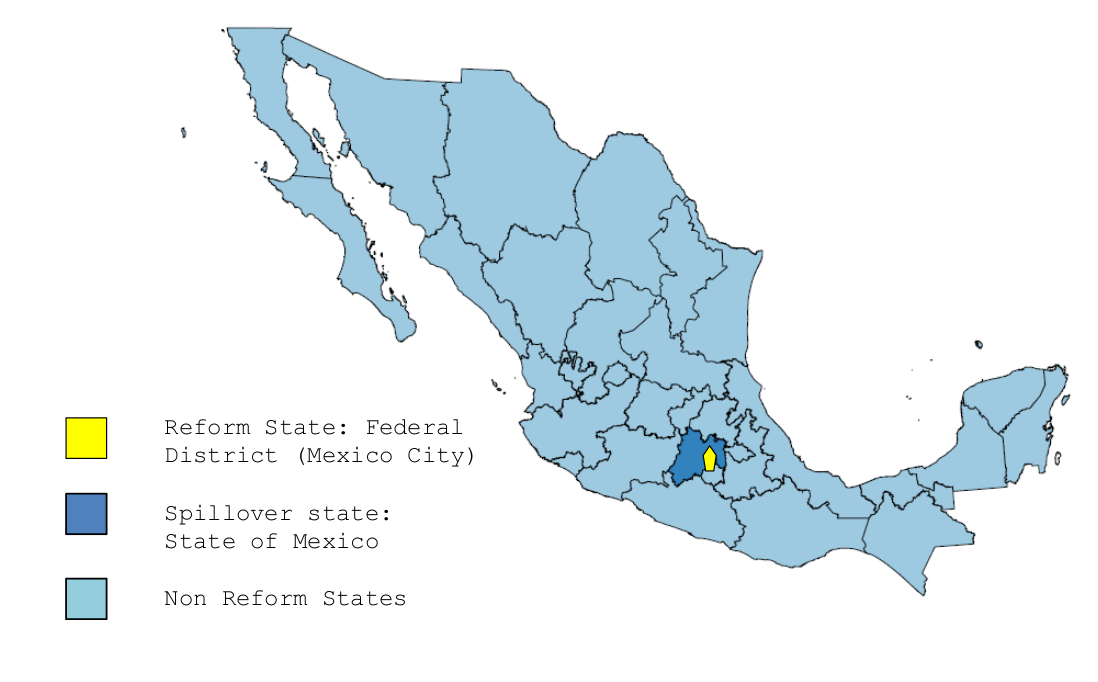
\includegraphics[scale=0.32]{./figures/MexReform.png}
\end{center}
\end{figure}
\end{frame}

\begin{frame}[label=ChileMap]
\begin{figure}
\begin{center}
\caption{Chile Reform Areas}
\hspace{-16mm}\includegraphics[scale=0.2]{./figures/Pill_l.eps}
\end{center}
\end{figure}
\end{frame}


%================================================================================
\section{Conclusion and Future Work}
\begin{frame}[label=concl]
  \frametitle{Conclusion and Future Work}

\end{frame}


\begin{frame}[label=future]
  \frametitle{Conclusion and Future Work}
\begin{itemize}
\item Current work using a historical well documented contraceptive reform in USA
\item Extension to a structural interpretation to motivate access to treatment
\item Stata module \texttt{cdifdif} (and full source code for this project) 
  available for download at \texttt{https://github.com/damiancclarke/spillovers/}
\end{itemize}
\end{frame}


\begin{frame}
{\Large Appendices}
\end{frame}

\begin{frame}[label=ChileDesc]
\begin{table}[htpb!] \centering
\caption{Summary Statistics} \label{TEENtab:SumStats}
\scalebox{0.42}{
\begin{tabular} {@{\extracolsep{5pt}}lp{3mm}ccc}\\ [-1.8ex]
\hline\hline\\ [-1.8ex] &&No Pill&Pill&Total \\
&&Available&Available& \\ \midrule 
\textsc{Municipality Characteristics}&&&& \\
&&&& \\
Poverty &&16.4&17.0&16.6\\
&&(7.47)&(7.56)&(7.49) \\
Conservative &&0.286&0.267&0.281\\
&&(0.452)&(0.443)&(0.45) \\
Education Spending &&4,817&5,980&5,108\\
&&(5,649)&(6,216)&(5,818) \\
Health Spending &&1,866&2,788&2,096\\
&&(2,635)&(3,381)&(2,867) \\
Out of School &&4.07&3.98&4.05\\
&&(3.16)&(3.06)&(3.13) \\
Female Mayor &&0.120&0.134&0.123\\
&&(0.325)&(0.341)&(0.329) \\
Female Poverty &&60.5&62.0&60.8\\
&&(10.64)&( 9.48)&(10.4) \\
Pill Distance &&5.94&0.00&4.46\\
&&(18.4)&( 0.0)&(16.1) \\
&&&& \\
\textsc{Individual Characteristics}&&&&\\
&&&& \\
Live Births &&0.054&0.053&0.054\\
&&(0.226)&(0.224)&(0.226) \\
Fetal Deaths &&0.0558&0.0513&0.0547\\
&&(0.269)&(0.256)&(0.266) \\
Birthweight &&3322.7&3334.3&3324.7\\
&&     (540.0)&     (542.3)&     (540.4)\\
Maternal education  &&       11.92&       12.03&       11.94\\
&&     (2.967)&     (2.894)&     (2.955)\\
Percent working     &&       0.295&       0.395&       0.312\\
&&     (0.456)&     (0.489)&     (0.463)\\
Married     &&       0.340&       0.309&       0.335\\
&&     (0.474)&     (0.462)&     (0.472)\\
Age at Birth      &&       27.05&       27.15&       27.07\\
&&     (6.777)&     (6.790)&     (6.779)\\ \midrule
N Comunas && 346 &280& 346 \\
N Fetal Deaths &&9,999&3,064&13,063\\
N Births &&1,214,088&391,212&1,605,300\\
\hline \hline \\[-1.8ex]
%\multicolumn{5}{p{12.0cm}}{\begin{footnotesize}\textsc{Notes:}
%Group means are presented with standard deviations below in
%parentheses.  Poverty refers to the \% of the municipality
%below the poverty line, conservative is a binary variable
%indicating if the mayor comes from a politically conservative
%party
%health and education spending are measured in thousands
%of Chilean
%pesos, and pill distance measures the distance (in km) to the
%nearest municipality which reports prescribing emergency
%contraceptives.  Pregnancies are reported as \% of all women
%giving live birth, while fetal deaths are reported per live
%birth.  All summary statistics are for the period 2006-2012.
%\end{footnotesize}} 
\normalsize\end{tabular}}\end{table}

\hyperlink{empirA}{\textcolor{blue}{Back}}
\end{frame}

\begin{frame}[label=MexicoDesc]
\begin{table}[htbp]\centering
\def\sym#1{\ifmmode^{#1}\else\(^{#1}\)\fi}
\caption{Descriptive Statistics (Mexico)}
\label{Stab:MexDescriptives}
\scalebox{0.75}{
\begin{tabular}{l*{1}{ccccc}}
\toprule
                    &       Observations&        Mean&          Std. Dev.&         Min.&         Max.\\
&&&&&\\
\midrule
Treatment    &       24550&        0.00&        0.04&           0&           1\\
Close to Treatment        &       24550&        0.00&        0.05&           0&           1\\
Number of Births (Mexico DF)&         160&    11744.75&     8835.83&        1550&       34729\\
Number of Births (Close to DF)&         250&    12419.40&     9254.72&        1550&       39745\\
Number of Births (Other Areas)&       24300&      785.99&     3153.99&           0&       86659\\
Year (2001-2010)               &       24550&     2005.50&        2.87&        2001&        2010\\
Number of Medical Staff&       24550&       57.97&      250.81&           0&        6212\\
Number of Classrooms&       24550&      303.51&     1000.80&           0&       19280\\
Number of Libraries &       24550&        4.27&       16.95&           0&         708\\
Municipal Income &       24550&       75.51&      254.56&           0&        6615\\
Municipal Spending &       24550&       82.71&      271.05&           0&        6615\\
Regional Unemployment Rate&       24550&        2.93&        1.46&           0&           9\\
\midrule
\multicolumn{6}{p{13.8cm}}{\begin{footnotesize}\textsc{Notes:} Observations are for 2,455 municipalities in
10 years.  Number of births refers to total counts for all women aged 15-49 in each municipality within
the given area.  Municipal income and municipal spending refer to tax receipts and outlays, and are expressed
in millions of pesos. \end{footnotesize}}\\ \bottomrule
\end{tabular}}
\end{table}

\end{frame}

\begin{frame}[label=empirA1]
%  \frametitle{Emergency Contraceptive Pill in Chile} 
\begin{figure}
\begin{center}
\caption{Birth Figures and ILE Use (Mexico)}
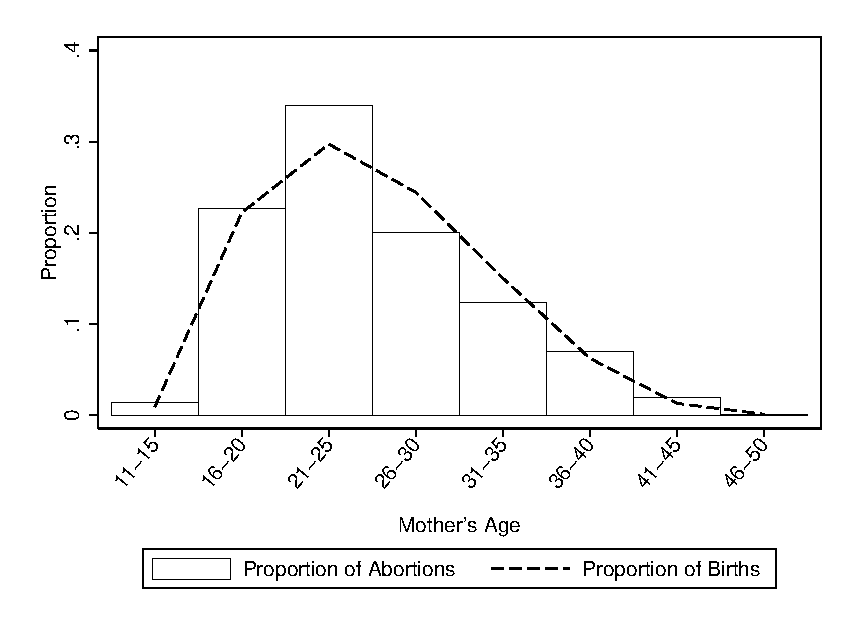
\includegraphics[scale=0.7]{./figures/birthDescriptives.eps}
\end{center}
\end{figure}
\hyperlink{empirB}{\textcolor{blue}{Back}}
\end{frame}


\begin{frame}[label=GrossEtAl]
\frametitle{Gross et al.\ (2014): EC in USA}
``This paper studies the effect of EC during a time period in which abortion was legal. 
The effect of EC might be very different [were] abortion to be illegal 
(Bailey, Guldi, \& Hershbein, 2013; Joyce, 2013).''
\vspace{6mm}
\begin{itemize}
\item Gross et al.\ explicitly consider the outside cost of abortion $A$
\item One may hyptohesise that $A_{Chile}>>A_{USA}$
\item From Gross et al.\ ``These costs and benefits [$A$] reflect not only the financial 
cost of abortion or pregnancy, but also stigma, opportunity cost, and psychic costs.''
\vspace{7mm}
\end{itemize}
\hyperlink{empirA3}{\textcolor{blue}{Back}}
\end{frame}

\end{document}

